\documentclass[11pt,a4paper]{article}
\usepackage[T1]{fontenc}
\usepackage[utf8]{inputenc}
\usepackage{lmodern}
\usepackage[margin=2.2cm]{geometry}
\usepackage{booktabs,graphicx,amsmath,xcolor,float,caption,array,longtable,enumitem,tabularx,multirow}
\usepackage{microtype,fancyhdr,titlesec}
\usepackage[colorlinks=true,linkcolor=blue!50!black,urlcolor=blue!50!black,citecolor=blue!50!black]{hyperref}

\makeatletter\g@addto@macro\UrlBreaks{\do\_\do\.}\makeatother
\graphicspath{{../metvar/}{../../../hists_zbzc_run3_metsplit/Summer22/plots/}}
\setlist{itemsep=2pt,topsep=4pt}
\captionsetup{font=small,labelfont=bf}
\setlength{\parskip}{4pt}
\setlength{\parindent}{0pt}

\pagestyle{fancy}
\fancyhf{}
\lhead{\small MET $>$ 50 GeV and JER smearing, Summer22 Z+jet}
\rhead{\small \thepage}
\renewcommand{\headrulewidth}{0.4pt}

% coloured boxes (no tcolorbox on this node)
\newcommand{\cbox}[3]{\par\medskip\noindent\fcolorbox{#1!65!black}{#1!7}{\parbox{\dimexpr\linewidth-2\fboxsep-2\fboxrule}{\textbf{#2}\\[2pt]#3}}\par\medskip}
\newcommand{\answer}[2]{\cbox{green}{#1}{#2}}
\newcommand{\finding}[2]{\cbox{blue}{#1}{#2}}
\newcommand{\open}[2]{\cbox{orange}{#1}{#2}}

\newcommand{\Zee}{Z$\to$ee}
\newcommand{\Zmm}{Z$\to\mu\mu$}
\newcommand{\pt}{$p_\mathrm{T}$}
\newcommand{\met}{$p_\mathrm{T}^\mathrm{miss}$}
\newcommand{\aeta}{$|\eta|$}

\begin{document}

\begin{titlepage}
\centering
\vspace*{2.5cm}
{\LARGE\bfseries The data/MC deficit at MET $>$ 50 GeV in Run 3 Z+jet events:\\[6pt]
is the JER counted twice, which jets cause it,\\[6pt] and does it matter for Z+b / Z+c?\par}
\vspace{1.2cm}
{\large Summer22 (2022 runs C--D), \Zee{} and \Zmm{} + jet, BTVNanoCommissioning \texttt{Zb\_Zc\_ratio} workflow\par}
\vspace{1.2cm}
{\large Pranjal Srivastava\par}
\vspace{0.4cm}
{\large 22 November 2026\par}
\vfill
\begin{minipage}{0.85\linewidth}
\small
This report answers the questions raised in the group meeting about the MET $>$ 50 GeV deficit:
whether the jet energy resolution (JER) smearing is already contained in the NanoAOD (so that we smear twice),
whether we can simply keep the JER off, which jets are responsible, and how much any of this changes the
b-tag / c-tag yields that enter the Z+b / Z+c ratio. All numbers are from 20 files per sample with statistical errors only.
Code, outputs and slides are in the fork \texttt{Pranjal-Srivastava-2023/BTVNanoCommissioning}, branch
\texttt{coffea\_machine} (commits 895342e and b6f34d0).
\end{minipage}
\vspace{1.5cm}
\end{titlepage}

\tableofcontents
\newpage

%======================================================================
\section{Summary}
%======================================================================

\textbf{The problem.} In Summer22 Z+jet events, data/MC is about 0.70 for 50 $<$ MET $<$ 100 GeV
(0.697 $\pm$ 0.029 in \Zee, 0.687 $\pm$ 0.020 in \Zmm), while it is 0.96--0.97 below 50 GeV.
Our analysis cuts at MET $<$ 50 GeV, so the region above the cut is a control region; but a 30\% deficit there
means that the MC MET is not right, and that could bias the events that pass the cut.
Earlier runs showed that switching the JER smearing off makes the deficit disappear (data/MC 0.96).

\textbf{The answers, in short.}
\begin{enumerate}
\item \textbf{The JER is not counted twice.} The NanoAOD jets and the NanoAOD PuppiMET contain the JEC only, no JER smearing
(three tests on a DY file, Section~\ref{sec:q1}). Our code starts from the raw jet \pt{} and from RawPuppiMET anyway,
so even a smeared NanoAOD value could not enter. We apply the JER once, in MC.
\item \textbf{Keeping the JER off is not what JME recommends.} The JME recipe smears the MC jets and propagates the smearing
into the type-1 MET, including the low-\pt{} CorrT1METJet jets. Our nominal setup (run A) does exactly this, step by step
(Section~\ref{sec:q2}). The two small differences between our code and the recipe change the MET by less than 1\%.
\item \textbf{About half of the deficit comes from soft forward jets.} The JER scale factor (SF) is 1.60 for
2.65 $<$ \aeta{} $<$ 2.853 and 1.64 for 2.853 $<$ \aeta{} $<$ 2.964, far larger than anywhere else (1.02--1.30).
Jets in that region, mostly with \pt{} $<$ 30 GeV, get a random smearing of about 75\% of their \pt{}, which kicks the MET.
This one region produces about half of the MC excess at MET 50--100 GeV (Section~\ref{sec:p1}).
\item \textbf{Measured directly with data:} removing the JER from the MET only for jets at 2.5 $<$ \aeta{} $<$ 3.139 moves
data/MC at MET 50--100 GeV from 0.70 to 0.82 (\Zee) and from 0.69 to 0.84 (\Zmm); removing it for all jets gives 0.95
(Section~\ref{sec:p2res}). The MC-only study had predicted 0.83 and 0.86.
\item \textbf{With no JER in the MET, the MC describes the MET shape:} data/MC is then flat at 0.94--0.95 below and above
50 GeV. The smearing does not change the number of MC events, it only moves them across the 50 GeV cut.
\item \textbf{Effect on the measurement is small.} The MC b-tag / c-tag yield ratio changes by less than 1\% at the Loose
working point and by up to about 3\% at Tight, which is about the size of the current data statistical error on that ratio
(Section~\ref{sec:bc}).
\item \textbf{Not fixed:} the MC hadronic recoil is wider than in data even with no JER at all
(RMS of $u_\perp$ at low $p_\mathrm{T}(\ell\ell)$: 13.9 GeV data, 15.7 GeV MC without JER, 17.0 GeV nominal MC),
and the recoil response differs by 1--2.5 GeV independently of the JER (Section~\ref{sec:recoil}).
\end{enumerate}

\textbf{Proposal.} Keep the JME recipe (run A) as the nominal setup. Use the change of the b/c ratio when the JER is
removed from the MET (for 2.5 $<$ \aeta{} $<$ 3.139, or for all jets, whichever is larger) as a systematic uncertainty
from the MET cut. Ask JME whether the 1.60--1.64 SF is meant to be used for jets below 30 GeV and for the low-\pt{}
jets that enter the MET.

\textbf{A correction to something said earlier.} The JER SF uncertainty in 2.65 $<$ \aeta{} $<$ 2.853 was quoted
in discussion as 1.60 $\pm$ 0.10. The correct value from the JSON file is a relative uncertainty of 9.6\%, i.e.
1.60 $\pm$ 0.15. The $-1\sigma$ value of 1.45 quoted at the time was correct.

%======================================================================
\section{Context}
%======================================================================

\subsection{The analysis and the MET cut}
We measure Z($\to\ell\ell$)+b / Z($\to\ell\ell$)+c in Run 3 with the \texttt{Zb\_Zc\_ratio} workflow.
Events have two same-flavour opposite-charge leptons with 71 $<$ m($\ell\ell$) $<$ 111 GeV, at least one AK4 PUPPI jet
with \pt{} $>$ 30 GeV and \aeta{} $<$ 2.5, and a type-1 PUPPI MET below 50 GeV. The MET cut removes $t\bar t$ events,
which have real neutrinos. The leading jet is b- or c-tagged with ParticleNet, DeepJet or RobustParT. The full setup
(triggers, IDs, SFs, weights) is in Appendix~\ref{app:setup}.

The quantity we eventually need is the ratio of b-tagged to c-tagged yields after corrections. A wrong MC MET
matters for that measurement only through the MET $<$ 50 GeV cut: if the MC MET is too wide, too many MC events are
removed by the cut, and if that loss depends on the jet flavour, the b/c ratio is biased.

\subsection{Definitions used throughout}
\begin{description}[leftmargin=2.8cm,style=nextline]
\item[All cuts except MET] the full selection (Z + jet), without the MET cut. This is where the MET distribution is shown.
\item[Full selection] all cuts, including MET $<$ 50 GeV.
\item[Z stage] trigger, two leptons, opposite charge, Z mass window; no jet and no MET requirement.
\item[data/MC] data yield divided by the MC prediction with all corrections and weights. Errors: statistical, data and MC.
\item[MET 50--100 fraction] fraction of events (all cuts except MET) with 50 $<$ MET $<$ 100 GeV.
\end{description}

\subsection{What was known before this study}
Three full runs (all with the MET XY correction and the DY $p_\mathrm{T}(\ell\ell)$ weights, 20 files per sample) were made on 16 November:
\begin{center}
\footnotesize
\begin{tabular}{l p{5.4cm} ccc}
\toprule
run & what is smeared & \multicolumn{3}{c}{data/MC, all cuts except MET, \Zee{} / \Zmm} \\
 & & MET $<$ 50 & MET 50--100 & MET 100--200 \\
\midrule
A (nominal) & JER for all jets and propagated into the MET & 0.971 / 0.964 & 0.697 / 0.687 & 0.917 / 0.750 \\
B & no JER at all (neither jets nor MET) & 0.959 / 0.952 & 0.964 / 0.961 & 1.27 / 1.02 \\
C & jets smeared as A; in the MET only gen-matched jets are smeared & 0.954 / 0.945 & 0.836 / 0.844 & -- \\
\bottomrule
\end{tabular}
\end{center}
So the JER, as propagated into the MET, causes most of the deficit. Run C showed that the random smearing of jets without a
generator jet is about half of it, and the other half comes from gen-matched jets. Run B, however, makes other things worse:
the \pt{} balance between the Z and the selected jet ($\chi^2$/ndf 40 $\to$ 58 in \Zee, 110 $\to$ 144 in \Zmm), so JER off is
not simply better. This report finds out which jets cause the effect and what it means for the measurement.

%======================================================================
\section{Background: JEC, JER and the type-1 MET}
\label{sec:bg}
%======================================================================

\subsection{Jet energy corrections (JEC)}
The JEC (here Summer22\_22Sep2023\_V4, L1L2L3Res for data, L1L2L3 for MC) scale the raw jet \pt{} so that, on average,
a reconstructed jet has the \pt{} of the particle-level jet. They correct the \emph{scale}, in data and MC.
For PUPPI jets there is no L1 pile-up offset (the L1 step is the identity), since PUPPI already removes pile-up particles.

\subsection{Jet energy resolution (JER) smearing}
The jet \pt{} resolution in data is worse than in simulation. To make MC look like data, the MC jets are smeared
by the \emph{hybrid method} (JME). With $s$ the data/MC resolution scale factor and $\sigma_\mathrm{MC}$ the MC relative resolution:
\begin{align}
\text{jet with a matching generator jet:}\quad & c = 1 + (s-1)\,\frac{p_\mathrm{T}-p_\mathrm{T}^\mathrm{gen}}{p_\mathrm{T}}, \\
\text{any other jet:}\quad & c = 1 + \mathcal{N}(0,\sigma_\mathrm{MC})\,\sqrt{\max(s^2-1,\,0)},
\end{align}
and the jet \pt{} becomes $c \cdot p_\mathrm{T}$. JME's matching requires $\Delta R < R/2 = 0.2$ and
$|p_\mathrm{T}-p_\mathrm{T}^\mathrm{gen}| < 3\sigma_\mathrm{MC}\,p_\mathrm{T}$. The scaling of matched jets stretches the
existing difference to the generator jet; the random smearing of unmatched jets adds a Gaussian of relative width
$\sigma_\mathrm{MC}\sqrt{s^2-1}$. JER smearing is applied only in MC.

\subsection{Type-1 PUPPI MET}
The raw MET is the negative vector sum of all PUPPI particles (\texttt{RawPuppiMET} in NanoAOD). The type-1 correction
replaces, for every jet, the raw jet momentum by the corrected one:
\begin{equation}
\vec{p}_\mathrm{T}^{\,\mathrm{miss,\,T1}} = \vec{p}_\mathrm{T}^{\,\mathrm{miss,\,raw}}
 - \sum_{\text{jets}} \left( \vec{p}_\mathrm{T}^{\,\mathrm{full}} - \vec{p}_\mathrm{T}^{\,\mathrm{L1}} \right),
\qquad p_\mathrm{T}^\mathrm{full} = p_\mathrm{T}^\mathrm{raw,\,no\,\mu}\times\mathrm{JEC}\times\mathrm{JER},
\end{equation}
where the muon energy is first removed from the jet (\texttt{muonSubtrFactor}), and $p_\mathrm{T}^\mathrm{L1}$ is the
muon-subtracted raw \pt{} (identity L1 for PUPPI). A jet enters the sum if its final \pt{} $>$ 15 GeV, \aeta{} $<$ 5.2
and its EM energy fraction $<$ 0.9. The jets are the NanoAOD \texttt{Jet} collection (\pt{} $>$ 15 GeV after the
production JEC) plus \texttt{CorrT1METJet}, the low-\pt{} jets stored only for the MET (raw \pt{} below the \texttt{Jet}
threshold). The CorrT1METJet jets have no link to generator jets, so in our code they always get the random smearing.

\textbf{Why the MET is so sensitive to the JER.} The MET is a vector sum. Each jet in the sum gets its own random
smearing, so the MET gets a random kick from every jet, mostly from many soft jets. The jets we select for the analysis
(\pt{} $>$ 30 GeV, \aeta{} $<$ 2.5) have small SFs and small smearing; the soft forward jets do not
(Section~\ref{sec:sf}).

%======================================================================
\section{Question 1: is the JER already in the NanoAOD?}
\label{sec:q1}
%======================================================================

\textbf{The hypothesis from the meeting.} If the NanoAOD \texttt{Jet\_pt} or \texttt{PuppiMET} were already
smeared, our smearing would come on top, the MC MET would be too wide, and switching our JER off would ``fix'' it.

\subsection{What our code starts from}
\begin{itemize}
\item Jets: raw \pt{} $= (1-\texttt{Jet\_rawFactor})\times\texttt{Jet\_pt}$, then our JEC, then our JER (MC only).
\item MET: starts from \texttt{RawPuppiMET} (the plain sum of the PUPPI particles), not from \texttt{PuppiMET}. The low-\pt{}
jets of the MET start from \texttt{CorrT1METJet\_rawPt}.
\end{itemize}
So even if a NanoAOD value were smeared, it would be undone before our corrections are applied: double counting is
impossible by construction. We still checked the files directly.

\subsection{Three tests on one Summer22 DY file (40\,000 events)}
\begin{center}
\small
\begin{tabular}{p{6.3cm} p{3.6cm} p{4.6cm}}
\toprule
test & if NanoAOD were smeared & what we find \\
\midrule
1. NanoAOD \texttt{Jet\_pt} / (raw \pt{} $\times$ our JEC) & random spread $\sim$9\% at 20 GeV & spread 0.3--0.9\% (\pt{} 15 $\to$ 100+ GeV) \\
2. width of jet \pt{} / gen-jet \pt, \aeta{} $<$ 1.3, gen \pt{} 20--30 / 50--100 GeV & SF $\times$ MC res.: 0.202 / 0.131 & 0.188 / 0.111 (MC res.\ 0.182 / 0.118) \\
3a. NanoAOD \texttt{PuppiMET} $-$ our type-1 MET (JEC only) & $\approx$ our MET with JER & median $+$0.06 GeV, width 1.3 GeV \\
3b. NanoAOD \texttt{PuppiMET} $-$ our type-1 MET (JEC + JER) & $\approx$ 0 & median $-$1.05 GeV, width 5.4 GeV \\
\bottomrule
\end{tabular}
\end{center}
\begin{itemize}
\item Test 1: the NanoAOD jet \pt{} equals raw \pt{} $\times$ JEC to better than 1\%, with no random component.
\item Test 2: the measured width matches the plain MC resolution, not the SF-inflated one.
\item Test 3: the NanoAOD PuppiMET agrees with our JEC-only type-1 MET (width 1.3 GeV, from the small differences in JEC
version and inputs), and disagrees with our JEC+JER MET (width 5.4 GeV).
\end{itemize}

\answer{Answer to Question 1: no double counting}{The NanoAOD jets and PuppiMET contain the JEC only, no JER smearing, and
our code starts from the raw values anyway. The JER smearing is applied exactly once, by us, in MC.}

%======================================================================
\section{Question 2: can we just keep the JER off?}
\label{sec:q2}
%======================================================================

The suggestion was: with the JER off, data/MC looks fine, so whatever is in the NanoAOD works. We read the JME documentation
(uploaded to \texttt{src/BTVNanoCommissioning/} in the repository) to see what is recommended.

\subsection{What the JME documentation says}
\textbf{Jet Energy Resolution page.} ``Measurements show that the JER in data is worse than in the simulation and the jets in MC
need to be smeared to describe the data.'' Apply the JEC first, then the JER, only in simulation. Hybrid method as in
Section~\ref{sec:bg}.

\textbf{Type-1 MET page and worked example (Type1MET.pdf).}
\begin{itemize}
\item ``Each jet receives the full JEC/JER chain before contributing to the MET update'': the JER smearing (MC) is one step of it.
\item The \texttt{Jet} and the \texttt{CorrT1METJet} collections are merged, and ``each jet is processed uniformly'', so the
CorrT1METJet jets are smeared too. A jet enters the MET if its final (smeared) \pt{} $>$ 15 GeV, \aeta{} $<$ 5.2, EM fraction $<$ 0.9.
\item The PuppiMET stored in the NanoAOD uses the JEC of the production; if the JEC changed, recompute it. This is why the
NanoAOD PuppiMET has no smearing: it is a starting point, not a recommendation to skip the smearing.
\end{itemize}

\subsection{Our type-1 MET compared with the recipe, step by step}
Code: \texttt{workflows/Zb\_Zc\_ratio.py} $\to$ \texttt{utils/correction.py} (\texttt{JME\_shifts}, \texttt{calc\_T1\_MET}).
The last column is the MC MET 50--100 fraction (or MET $>$ 50) with JER divided by that without JER, on the same events.
\begin{center}
\small
\begin{tabular}{p{7.4cm} p{3.0cm} p{4.4cm}}
\toprule
recipe step & in our code & effect on MC MET (tested) \\
\midrule
raw jet \pt, muon-subtracted & yes & \\
L1 offset: identity for PUPPI & yes & \\
JEC L1L2L3(Res), Summer22\_22Sep2023\_V4 & yes & \\
JER smearing (MC), Summer22\_22Sep2023\_JRV2 & yes & \\
Jet + CorrT1METJet merged, both smeared & yes & \\
selection: smeared \pt{} $>$ 15, \aeta{} $<$ 5.2, EM fraction $<$ 0.9 & yes & \\
MET shift $\sum(p_\mathrm{T}^\mathrm{full}-p_\mathrm{T}^\mathrm{L1})$ & yes & \\
unclustered uncertainty as a vector shift (Type1METUnc.pdf) & yes & \\
\midrule
gen matching $\Delta R<0.2$ and $3\sigma$ & no: any NanoAOD genJetIdx & MET $>$ 50 fraction $\times$1.075 $\to$ $\times$1.068 \\
JEC evaluated at raw \pt{} (JME talk, 2 Feb 2026) & at muon-subtracted \pt & no change: $\times$1.368 vs $\times$1.368 \\
CorrT1METJet matched to GenJets by $\Delta R$ & not done & no change: $\times$1.075 $\to$ $\times$1.075 \\
\bottomrule
\end{tabular}
\end{center}
The JER itself changes the MET 50--100 fraction by about 40\%; the deviations from the recipe change it by less than 1\%.

\subsection{Two JME talks of 2 February 2026}
\textbf{N.~Norjoharuddeen, ``MET Type-1 correction with NanoAODs'' (JME General).} Step-by-step recipe that reproduces CMSSW,
JEC only (no JER). Closure: the recomputed MET is within 0.5\% of PuppiMET for 99.9999\% of events (Summer24). The talk evaluates
the JEC at the raw jet \pt{} and applies it to the muon-subtracted \pt; we evaluate it at the muon-subtracted \pt. Tested: no
effect on our MET (table above).

\textbf{M.~Malucchi, ``Run 3 MET performance'' (DPG-PH JetMET), \Zmm{} DY MC only, no JER, no data.}
For 2022 NanoAODv12, the type-1 MET recomputed with JEC has a worse resolution and a larger high-MET tail than the stored
PuppiMET (``when re-applying the JEC for 2022 the MET resolution gets worse than PuppiMET; for 2023 this effect is much smaller'').
``DYJetsToLL\_M-50\_Nanov12\_2022preEE and DYto2L-4Jets\_MLL-50\_Nanov12\_preEE seem problematic for the MET resolution''; the
NanoAODv15 version does not show it. In our files, the stored PuppiMET has $\times$1.06 (\Zee) / $\times$1.10 (\Zmm) the MET
50--100 fraction of our JEC-only MET, while the JER gives $\times$1.37 / $\times$1.39: for us the JER is the larger effect. Their
remark about the 2022 v12 DY MET could be part of what stays even with the JER off (Section~\ref{sec:recoil}); not tested.

\answer{Answer to Question 2: switching the JER off is not what JME recommends}{The recipe smears the MC jets and propagates the
smearing into the type-1 MET. Our nominal run (A) does exactly that. Run B (JER off) and the MET versions in this report are
tests to locate the problem, not a recommended setup. Switching the JER off also makes the Z--jet \pt{} balance worse (Section 2.3).}

%======================================================================
\section{Phase 1 (MC only): which jets make the MC MET grow under JER?}
\label{sec:p1}
%======================================================================

\subsection{Method}
Script \texttt{study\_zbzc\_met\_jer\_split.py}, 65 DY files (stitched in generator $p_\mathrm{T}(\ell\ell)$ as in the workflow),
pile-up weights, simplified selection (no lepton SFs). For the same events, the type-1 MET is built about 30 times, each time
applying the JER in the MET sum only to one class of jets (by collection, gen matching, \pt, \aeta), and compared with
the MET without any JER. The number quoted is
\begin{equation}
R = \frac{\text{MC MET 50--100 fraction with JER for this class only}}{\text{MC MET 50--100 fraction with no JER in the MET}},
\end{equation}
so $R=1$ means that this class of jets does not change the MET. Check: all jets smeared gives $R$ = 1.37 (\Zee) and 1.39 (\Zmm);
in the full runs, data/MC went from 0.70 (JER on) to 0.96 (JER off), a factor 1.38. The simple study reproduces the effect.

\subsection{Results}
\begin{center}
\small
\begin{tabular}{l cc}
\toprule
JER applied in the MET only to \ldots{} (all cuts except MET) & \Zee & \Zmm \\
\midrule
all jets (= run A) & 1.368 & 1.390 \\
\midrule
Jet collection only & 1.251 & 1.257 \\
CorrT1METJet only & 1.125 & 1.124 \\
\midrule
gen-matched Jet only (= run C) & 1.116 & 1.122 \\
unmatched Jet only & 1.113 & 1.129 \\
\midrule
\pt{} 0--20 GeV only & 1.174 & 1.196 \\
\pt{} 20--30 GeV only & 1.063 & 1.066 \\
\pt{} 30--50 GeV only & 1.040 & 1.038 \\
\pt{} $>$ 50 GeV only & 1.078 & 1.076 \\
\midrule
\aeta{} 0--1.3 only & 1.041 & 1.043 \\
\aeta{} 1.3--2.5 only & 1.075 & 1.059 \\
\aeta{} 2.5--3.0 only & 1.211 & 1.254 \\
\aeta{} 3.0--5.2 only & 1.037 & 1.020 \\
\midrule
\pt{} $<$ 30 and \aeta{} $>$ 2.5 only & 1.218 & 1.245 \\
\pt{} $<$ 30 and \aeta{} $<$ 2.5 only & 1.026 & 1.021 \\
\pt{} $>$ 30 and \aeta{} $<$ 2.5 only (type of jets we select) & 1.081 & 1.075 \\
\pt{} $>$ 30 and \aeta{} $>$ 2.5 only & 1.030 & 1.038 \\
\midrule
\aeta{} 2.5--2.65 only (SF 1.22) & 1.017 & 1.023 \\
\textbf{\aeta{} 2.65--2.853 only (SF 1.60)} & \textbf{1.179} & \textbf{1.203} \\
\aeta{} 2.853--2.964 only (SF 1.64) & 1.022 & 1.031 \\
\aeta{} 2.964--3.139 only (SF 1.21) & 1.007 & 1.006 \\
\midrule
all except \aeta{} 2.65--2.964 & 1.176 & 1.153 \\
all except \aeta{} 2.5--3.139 & 1.157 & 1.119 \\
\midrule
JEC at raw \pt{} (JME talk), JER all & 1.368 & 1.390 \\
NanoAOD PuppiMET as stored (vs our JEC-only MET) & 1.064 & 1.097 \\
\bottomrule
\end{tabular}
\end{center}

\begin{figure}[H]
\centering
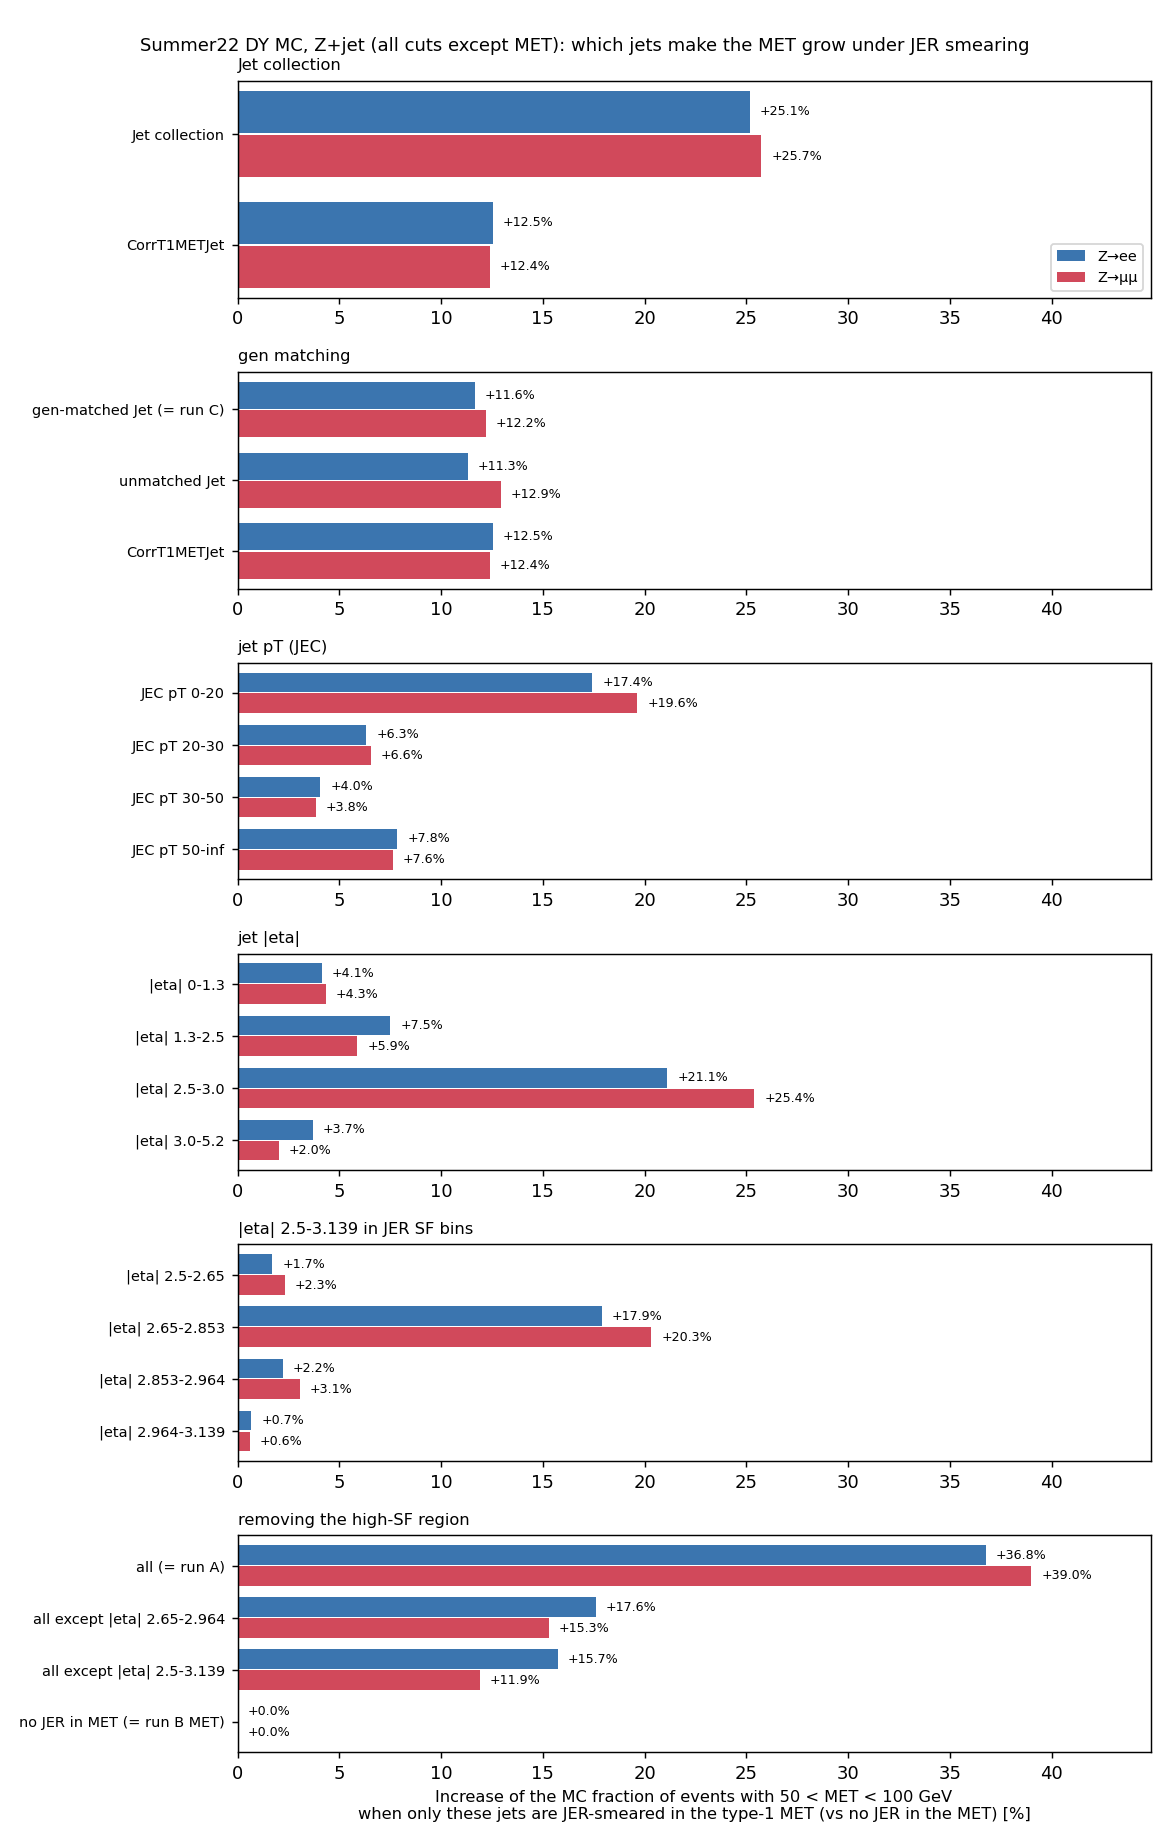
\includegraphics[width=\linewidth]{met_jer_split_zjet.png}
\caption{Phase 1, MC only, all cuts except MET: increase of the MC MET 50--100 fraction, $100\times(R-1)$, when only the jets
named on the left are JER-smeared in the type-1 MET. Blue \Zee, red \Zmm. Same x scale in all panels.}
\label{fig:p1}
\end{figure}

\finding{What Phase 1 shows}{
\begin{itemize}[leftmargin=12pt]
\item One \aeta{} bin, 2.65--2.853, alone gives $R$ = 1.18--1.20, about half of the full 1.37--1.39.
\item The effect is in soft jets: \pt{} $<$ 30 GeV and \aeta{} $>$ 2.5 gives 1.22--1.25; the type of jets we select gives only 1.08.
\item Gen-matched and unmatched jets contribute equally (1.12 / 1.11--1.13): it is not only pile-up jets without a generator jet.
\item The rest of the effect is spread over all other jets; no other single class gives more than $R \approx 1.08$.
\item Neither the JEC evaluation point nor the stored-PuppiMET choice is the cause.
\end{itemize}
Prediction for data: if the JER is removed from the MET for 2.5 $<$ \aeta{} $<$ 3.139, data/MC at MET 50--100 should become
about 0.964/1.157 = 0.83 (\Zee) and 0.961/1.119 = 0.86 (\Zmm).}

\subsection{Why that \aeta{} region: the Summer22 JER scale factors}
\label{sec:sf}
\texttt{Summer22\_22Sep2023\_JRV2\_MC\_ScaleFactor\_AK4PFPuppi} (below 121 GeV one value per \aeta{} bin) and the MC resolution at $\rho = 20$:
\begin{center}
\small
\begin{tabular}{l c c c c}
\toprule
\aeta & JER SF & SF uncertainty (relative) & SF $-1\sigma$ & MC resolution at 15 / 100 GeV \\
\midrule
0 -- 1.305 & 1.06 -- 1.13 & 1.5 -- 2.2\% & 1.03 -- 1.11 & 16--24\% / 10--12\% \\
1.305 -- 2.5 & 1.02 -- 1.30 & 3 -- 12\% & 0.92 -- 1.22 & 28--44\% / 12--13\% \\
2.5 -- 2.65 & 1.22 & 5.9\% & 1.15 & 56\% / 13\% \\
\textbf{2.65 -- 2.853} & \textbf{1.60} & \textbf{9.6\%} & \textbf{1.45} & \textbf{60\% / 14\%} \\
\textbf{2.853 -- 2.964} & \textbf{1.64} & \textbf{16.9\%} & \textbf{1.36} & \textbf{75\% / 16\%} \\
2.964 -- 3.139 & 1.21 & 11.8\% & 1.06 & 52\% / 19\% \\
3.139 -- 5.191 & 1.12 & 13.4\% & 0.97 & 35--38\% / 9--11\% \\
\bottomrule
\end{tabular}
\end{center}
For an unmatched jet the random smearing has a relative width $\sigma_\mathrm{MC}\sqrt{s^2-1}$. With $s = 1.6$ and
$\sigma_\mathrm{MC} = 60\%$ at 15 GeV this is $0.60\times\sqrt{1.6^2-1} = 0.60\times1.25 \approx 75\%$ of the jet \pt.
For a central jet ($s = 1.1$, $\sigma_\mathrm{MC} = 20\%$) it is $0.20\times0.46 \approx 9\%$. For matched jets the scaling by
$(s-1) = 0.6$ of the existing difference to the generator jet is also large, because the resolution itself is 60\% there.

Even at $-1\sigma$ the SFs are 1.45 and 1.36 (widths of about 63\% and 69\% at 15 GeV): the quoted SF uncertainty cannot
cover the difference to the data. The narrower 2.853--2.964 bin, despite the larger SF, contributes only 2--3\%; we did not
study why.

%======================================================================
\section{Phase 2: the MET in seven versions in one full run}
\label{sec:p2}
%======================================================================

\subsection{Why a second phase}
Phase 1 is MC only, with a simplified selection. To get data/MC directly, with the full analysis (all SFs, weights, MET XY
correction, tag regions), we made one new run in which the MET is filled in several versions side by side.

\subsection{The versions}
Run \texttt{zbzc\_run3\_metvar}, workflow \texttt{Zb\_Zc\_ratio\_metvar} = run A (MET XY correction, DY $p_\mathrm{T}(\ell\ell)$
weights, 20 files per sample) with the option \texttt{met\_variants=True}. Only the MET changes; the selected jets are smeared
as in run A in every version, so the jet selection and the jet \pt{} are identical.
\begin{center}
\small
\begin{tabular}{l l}
\toprule
version & what is different (MC only) \\
\midrule
nominal (= run A) & JER for all jets in the MET \\
no JER 2.65--2.964 & no JER in the MET for jets with 2.65 $<$ \aeta{} $<$ 2.964 (the two high-SF bins) \\
no JER 2.5--3.139 & no JER in the MET for jets with 2.5 $<$ \aeta{} $<$ 3.139 \\
no JER soft \& 2.5--3.139 & no JER in the MET for jets with \pt{} $<$ 30 GeV and 2.5 $<$ \aeta{} $<$ 3.139 \\
no JER \pt{} $<$ 30 & no JER in the MET for jets with \pt{} $<$ 30 GeV (all \aeta) \\
no JER CorrT1 & no JER in the MET for the CorrT1METJet jets \\
no JER in MET & no JER in the MET at all \\
run B (for comparison) & no JER anywhere (jets and MET), separate earlier run \\
\bottomrule
\end{tabular}
\end{center}

\subsection{How it is done}
The workflow intercepts the framework's own call to the JER function for the type-1 jets (\texttt{get\_JER} in
\texttt{correction.py}), keeps those jets and their JER factors, and redoes the type-1 sum with the factor set to 1 for one class
of jets. The jet selection for the MET sum (smeared \pt{} $>$ 15 GeV) uses the \pt{} of that version. The MET XY correction is
then applied to every version in the same way, and every version is filled in the same histograms as the nominal MET (all
tag regions) and in recoil histograms. \pt{} and \aeta{} classes use the JEC-corrected \pt{} and the jet \aeta.

Data have no JER, so the data MET is the same in every version; data were not rerun, and the data histograms of run A are used.

\subsection{Validation}
\begin{itemize}
\item All 9 MC samples (5 DY \pt-bins, $t\bar t$, WW, WZ, ZZ) processed 20/20 files. The stall watchdog killed one sample
(DY $p_\mathrm{T}(\ell\ell)$ 400--600) twice; the third attempt finished normally.
\item The version ``all'' recomputed by the new code equals the framework MET: 0 of 2\,797\,218 Z events differ by more than 0.01 GeV.
\item The MC MET histogram of version ``all'' equals run A's histogram exactly (maximum relative difference 0).
\item A one-file test before the run gave the same result (sum of $|$differences$|$ $\sim 10^{-11}$ GeV).
\end{itemize}

%======================================================================
\section{Phase 2 results}
\label{sec:p2res}
%======================================================================

\subsection{data/MC per MET bin}
\begin{center}
\footnotesize
\begin{tabular}{l l ccc c}
\toprule
 & version & MET $<$ 50 & MET 50--100 & MET 100--200 & MC 50--100 / nom. \\
\midrule
\multirow{8}{*}{\Zee}
& nominal (A) & 0.971 $\pm$ 0.013 & 0.697 $\pm$ 0.029 & 0.917 $\pm$ 0.130 & 1.000 \\
& no JER 2.65--2.964 & 0.956 $\pm$ 0.012 & 0.814 $\pm$ 0.035 & 1.080 $\pm$ 0.145 & 0.856 \\
& no JER 2.5--3.139 & 0.955 $\pm$ 0.012 & 0.823 $\pm$ 0.035 & 1.147 $\pm$ 0.157 & 0.847 \\
& no JER soft \& 2.5--3.139 & 0.958 $\pm$ 0.012 & 0.797 $\pm$ 0.034 & 1.007 $\pm$ 0.137 & 0.875 \\
& no JER \pt{} $<$ 30 & 0.954 $\pm$ 0.012 & 0.838 $\pm$ 0.036 & 0.994 $\pm$ 0.136 & 0.832 \\
& no JER CorrT1 & 0.961 $\pm$ 0.012 & 0.768 $\pm$ 0.032 & 0.946 $\pm$ 0.131 & 0.907 \\
& no JER in MET & 0.944 $\pm$ 0.012 & 0.954 $\pm$ 0.043 & 1.249 $\pm$ 0.168 & 0.731 \\
& run B & 0.959 $\pm$ 0.012 & 0.964 $\pm$ 0.043 & 1.274 $\pm$ 0.172 & 0.723 \\
\midrule
\multirow{8}{*}{\Zmm}
& nominal (A) & 0.964 $\pm$ 0.009 & 0.687 $\pm$ 0.020 & 0.750 $\pm$ 0.067 & 1.000 \\
& no JER 2.65--2.964 & 0.947 $\pm$ 0.009 & 0.822 $\pm$ 0.025 & 0.924 $\pm$ 0.083 & 0.836 \\
& no JER 2.5--3.139 & 0.945 $\pm$ 0.009 & 0.844 $\pm$ 0.026 & 0.912 $\pm$ 0.082 & 0.814 \\
& no JER soft \& 2.5--3.139 & 0.948 $\pm$ 0.009 & 0.816 $\pm$ 0.025 & 0.890 $\pm$ 0.079 & 0.842 \\
& no JER \pt{} $<$ 30 & 0.945 $\pm$ 0.009 & 0.853 $\pm$ 0.027 & 0.918 $\pm$ 0.082 & 0.806 \\
& no JER CorrT1 & 0.955 $\pm$ 0.009 & 0.754 $\pm$ 0.023 & 0.808 $\pm$ 0.072 & 0.912 \\
& no JER in MET & 0.937 $\pm$ 0.009 & 0.948 $\pm$ 0.031 & 0.982 $\pm$ 0.087 & 0.725 \\
& run B & 0.952 $\pm$ 0.009 & 0.961 $\pm$ 0.032 & 1.022 $\pm$ 0.091 & 0.715 \\
\bottomrule
\end{tabular}
\end{center}
The data are the same in every row, so the rows differ only through the MC, and their errors are strongly correlated.
The last column is the MC yield at MET 50--100 relative to the nominal MC.

\begin{figure}[H]
\centering
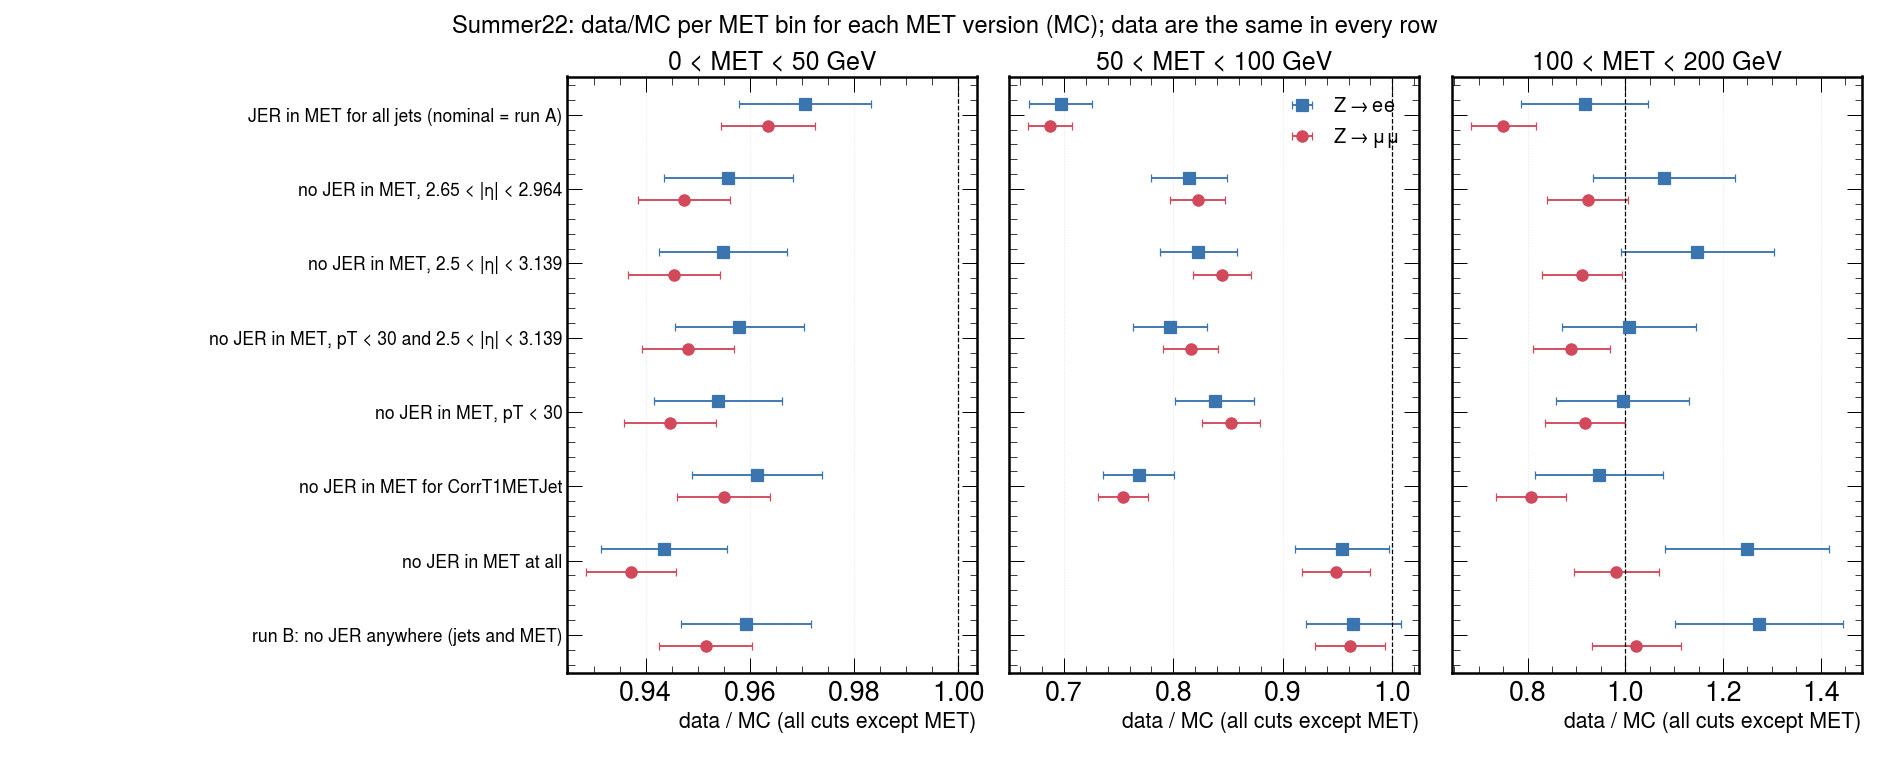
\includegraphics[width=\linewidth]{datamc_metbins.png}
\caption{data/MC per MET bin (all cuts except MET) for every MET version. Squares \Zee, circles \Zmm. Top row = nominal.
The data are the same in every row; only the MC MET changes. Note the different x ranges of the three panels.}
\label{fig:metbins}
\end{figure}

\begin{figure}[H]
\centering
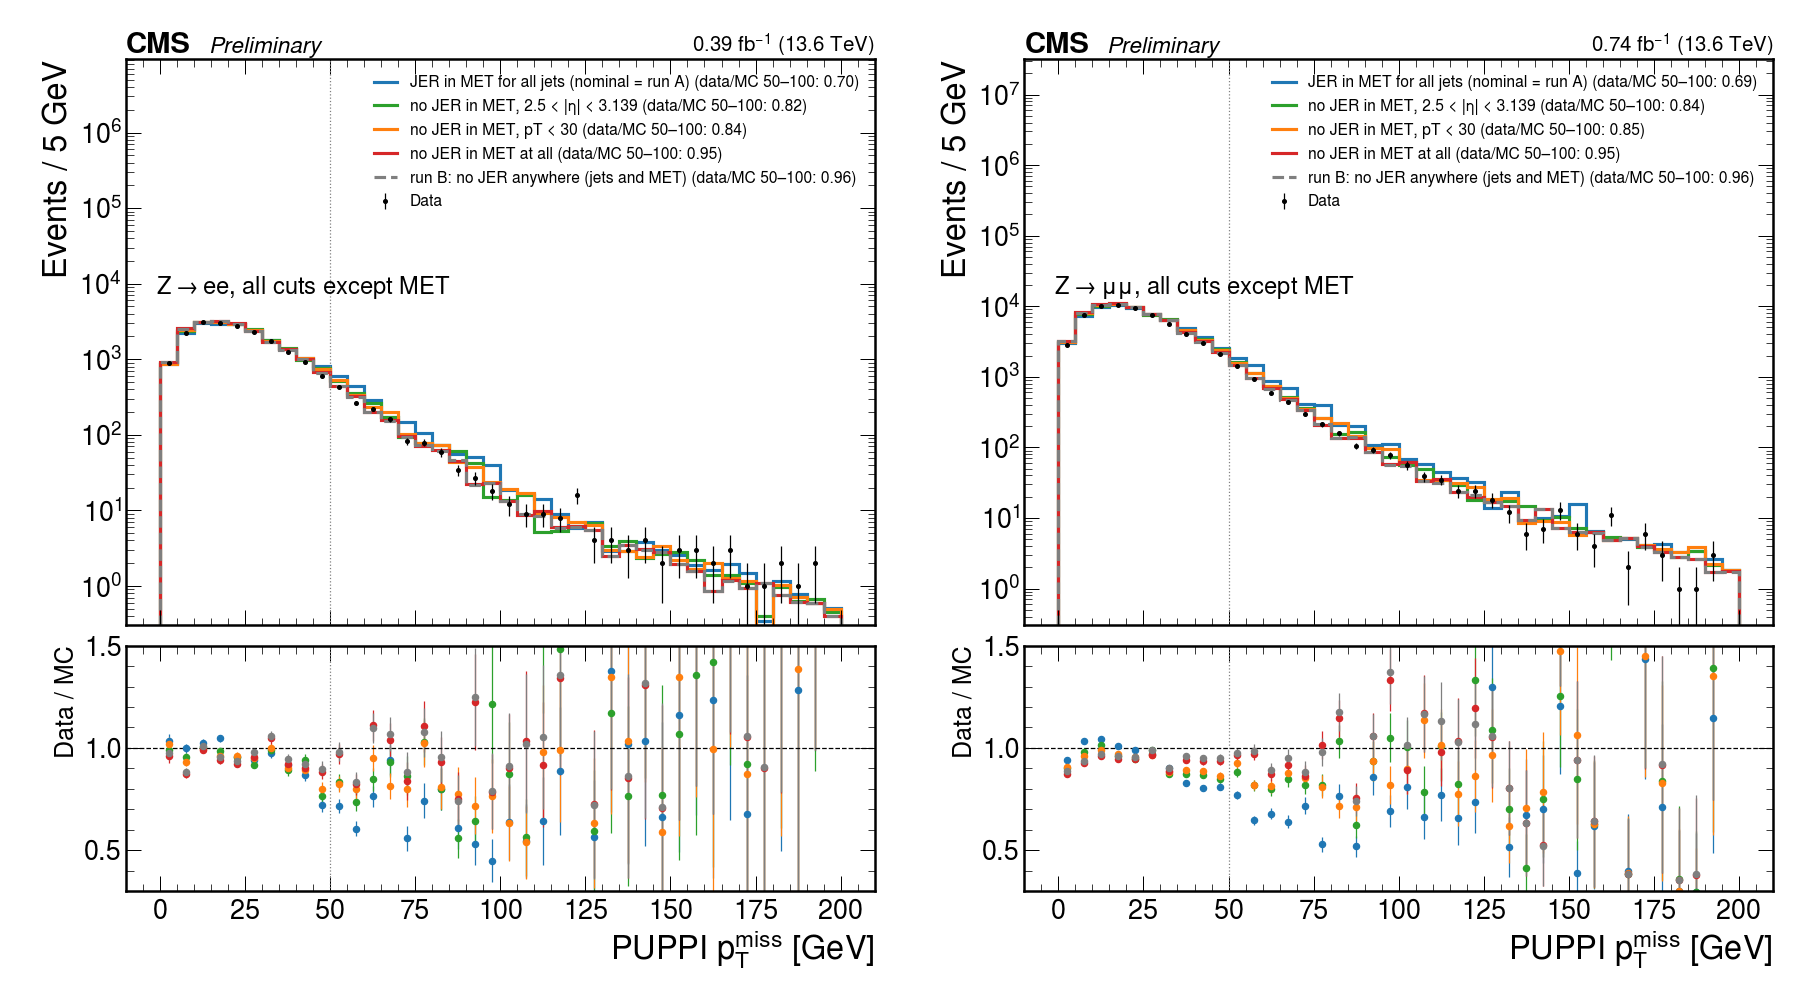
\includegraphics[width=\linewidth]{met_nm1_versions.png}
\caption{MET distribution, all cuts except MET. Black: data. Coloured: MC with the JER removed from the MET for the jets given in
the legend; dashed grey: run B. Lower panel: data/MC. Dotted line: the MET $<$ 50 GeV cut.}
\label{fig:metdist}
\end{figure}

\finding{What the MET bins show}{
\begin{itemize}[leftmargin=12pt]
\item Removing the JER from the MET for the two high-SF bins alone (2.65--2.964) closes about half of the gap at MET 50--100:
0.70 $\to$ 0.81 of 0.70 $\to$ 0.95 in \Zee{} (46\%), 0.69 $\to$ 0.82 of 0.69 $\to$ 0.95 in \Zmm{} (52\%).
\item 2.5--3.139: 0.82 / 0.84, consistent with the Phase 1 prediction (0.83 / 0.86).
\item All jets below 30 GeV: 0.84 / 0.85, a bit more than the forward region alone.
\item CorrT1METJet only: 0.77 / 0.75, a smaller part.
\item No JER in the MET: 0.95 / 0.95, the same as run B (0.96 / 0.96). The remaining 1\% difference, within the errors, would come from
the selected jets, which run B also leaves unsmeared.
\item Above 100 GeV the errors are 7--17\%; no version can be singled out there.
\end{itemize}}

\subsection{Below the cut: why data/MC at MET $<$ 50 changes}
At MET $<$ 50 GeV, data/MC goes from 0.971 / 0.964 (nominal) to 0.955 / 0.945 (no JER 2.5--3.139) and 0.944 / 0.937
(no JER in MET). The total number of MC events is the same in every version; the smearing only moves events from below 50 GeV
to above. With less smearing, more MC events stay below the cut, the MC prediction there grows by 1.5--2.7\%, and data/MC drops.

Seen the other way round, with no JER in the MET data/MC is flat in MET, 0.94--0.95 below and between 50 and 100 GeV. The
MC then describes the MET shape, and what is left is an overall normalisation difference of about 5\%, the same in all versions.
That normalisation difference is not studied in this report (it involves the luminosity of the 20-file sample, the lepton and
trigger SFs and the cross sections). The nominal 0.97 below the cut is closer to 1 partly because too many MC events leave
across the cut.

\subsection{Full selection per tag region}
data/MC at the full selection (MET $<$ 50 + jet), all weights, ParticleNet tag regions of the leading jet:
\begin{center}
\small
\begin{tabular}{l l ccccccc}
\toprule
 & version & incl & b L & c L & b M & c M & b T & c T \\
\midrule
\multirow{8}{*}{\Zee}
& nominal (A) & 0.971 & 0.973 & 0.952 & 0.984 & 0.964 & 1.033 & 0.943 \\
& no JER 2.65--2.964 & 0.956 & 0.953 & 0.937 & 0.958 & 0.952 & 1.009 & 0.924 \\
& no JER 2.5--3.139 & 0.955 & 0.952 & 0.936 & 0.952 & 0.952 & 1.003 & 0.925 \\
& no JER soft \& 2.5--3.139 & 0.958 & 0.957 & 0.940 & 0.957 & 0.956 & 1.009 & 0.928 \\
& no JER \pt{} $<$ 30 & 0.954 & 0.953 & 0.936 & 0.948 & 0.953 & 0.998 & 0.924 \\
& no JER CorrT1 & 0.961 & 0.962 & 0.943 & 0.967 & 0.959 & 1.012 & 0.937 \\
& no JER in MET & 0.944 & 0.942 & 0.925 & 0.935 & 0.940 & 0.990 & 0.910 \\
& run B & 0.959 & 0.961 & 0.942 & 0.945 & 0.950 & 0.996 & 0.914 \\
\midrule
\multirow{8}{*}{\Zmm}
& nominal (A) & 0.964 & 0.943 & 0.948 & 0.933 & 0.947 & 0.896 & 0.927 \\
& no JER 2.65--2.964 & 0.947 & 0.932 & 0.933 & 0.927 & 0.931 & 0.902 & 0.904 \\
& no JER 2.5--3.139 & 0.945 & 0.928 & 0.931 & 0.923 & 0.928 & 0.899 & 0.901 \\
& no JER soft \& 2.5--3.139 & 0.948 & 0.932 & 0.933 & 0.927 & 0.930 & 0.902 & 0.905 \\
& no JER \pt{} $<$ 30 & 0.945 & 0.927 & 0.930 & 0.921 & 0.927 & 0.899 & 0.902 \\
& no JER CorrT1 & 0.955 & 0.936 & 0.940 & 0.930 & 0.937 & 0.898 & 0.918 \\
& no JER in MET & 0.937 & 0.918 & 0.923 & 0.911 & 0.919 & 0.889 & 0.893 \\
& run B & 0.952 & 0.933 & 0.938 & 0.916 & 0.929 & 0.892 & 0.898 \\
\bottomrule
\end{tabular}
\end{center}
Statistical errors: about $\pm$0.012 (incl), $\pm$0.03 (Loose), $\pm$0.05 (Medium), $\pm$0.07 (Tight) in \Zee; about 25\% smaller
in \Zmm. In every tag region the versions move together by 1--3\%, as the inclusive selection does: the change is mostly
a normalisation change from the MET cut, not a change specific to b or c jets.

\subsection{Effect on the b-tag / c-tag yield ratio}
\label{sec:bc}
The quantity closest to the Z+b / Z+c ratio is the MC b-tag yield divided by the c-tag yield at the full selection.
Its change with respect to the nominal MET, in \%:
\begin{center}
\footnotesize
\setlength{\tabcolsep}{2.5pt}
\begin{tabular}{l ccccccc cc}
\toprule
 & \multicolumn{7}{c}{change in \% (no JER in the MET for \ldots)} & \multicolumn{2}{c}{b/c ratio} \\
 & 2.65--2.964 & 2.5--3.139 & soft, 2.5--3.1 & \pt{} $<$ 30 & CorrT1 & all & run B & nominal & data \\
\midrule
\Zee, L & $+0.6\pm0.4$ & $+0.5\pm0.4$ & $+0.3\pm0.4$ & $+0.4\pm0.4$ & $+0.3\pm0.3$ & $+0.4\pm0.5$ & $+0.2\pm4.2$ & 0.189 & 0.193 \\
\Zee, M & $+1.5\pm0.7$ & $+2.0\pm0.8$ & $+1.9\pm0.7$ & $+2.5\pm0.8$ & $+1.2\pm0.5$ & $+2.7\pm0.9$ & $+2.6\pm7.1$ & 0.209 & 0.213 \\
\Zee, T & $+0.4\pm1.0$ & $+1.0\pm1.1$ & $+0.8\pm1.0$ & $+1.4\pm1.1$ & $+1.4\pm0.8$ & $+0.6\pm1.4$ & $+0.4\pm10.4$ & 0.424 & 0.464 \\
\Zmm, L & $-0.5\pm0.2$ & $-0.3\pm0.2$ & $-0.4\pm0.2$ & $-0.3\pm0.3$ & $-0.2\pm0.2$ & $-0.1\pm0.3$ & $-0.1\pm3.2$ & 0.200 & 0.199 \\
\Zmm, M & $-1.1\pm0.3$ & $-1.0\pm0.3$ & $-1.2\pm0.3$ & $-0.9\pm0.4$ & $-0.8\pm0.2$ & $-0.6\pm0.5$ & $-0.1\pm5.5$ & 0.210 & 0.207 \\
\Zmm, T & $-3.1\pm0.4$ & $-3.1\pm0.4$ & $-3.0\pm0.4$ & $-3.0\pm0.4$ & $-1.1\pm0.3$ & $-2.9\pm0.6$ & $-2.7\pm7.9$ & 0.485 & 0.469 \\
\bottomrule
\end{tabular}
\end{center}
\textbf{About the errors.} The versions share the same MC events, so the error of a change is not the full MC error. Only the
events that cross the MET cut contribute; the approximate variance used is $|\sum w^2(\text{version}) - \sum w^2(\text{nominal})|$
for the b-tag and the c-tag yields. Run B is a different run with different jets, so its full MC statistical error is used.
For comparison, the data statistical error of the ratio is 1.9 / 3.3 / 4.8\% (\Zee) and 1.1 / 1.8 / 2.7\% (\Zmm) for L / M / T.

\finding{The MET choice moves the MC b/c-tag ratio by at most about 3\%}{
Loose: below 0.6\% in both channels. Medium: $+1.2$ to $+2.7$\% in \Zee{} and $-0.6$ to $-1.2$\% in \Zmm, with opposite signs,
so not a common shift of the physics. Tight: up to $+1.4$\% in \Zee{} and about $-3$\% in \Zmm{} (significant against its own
approximate error of 0.4\%, and about equal to the data statistical error of 2.7\%). Interestingly, at Tight in \Zmm{} the
versions with less smearing move the MC ratio (0.485) towards the data (0.469), but at this precision this is not a conclusion.}

%======================================================================
\section{Hadronic recoil}
\label{sec:recoil}
%======================================================================

\subsection{Definitions}
The recoil is everything in the event except the two leptons: $\vec u = -(\vec p_\mathrm{T}^{\,\mathrm{miss}} + \vec p_\mathrm{T}(\ell\ell))$.
It is split into a component along the Z direction, $u_\parallel$, and one perpendicular to it, $u_\perp$. With $q_\mathrm{T} = p_\mathrm{T}(\ell\ell)$:
\begin{itemize}
\item $\langle u_\parallel + q_\mathrm{T}\rangle$ is the \emph{response}: 0 if the recoil balances the Z exactly; positive if the
recoil is measured too small.
\item RMS($u_\perp$) is the \emph{resolution}: there is no true recoil perpendicular to the Z, so its spread is pure resolution
(pile-up, unclustered energy, jet resolution).
\end{itemize}
Histograms are filled for $|u| < 100$ GeV, so the RMS ignores the far tails. The recoil is shown at the Z stage (no jet, no MET cut)
and with all cuts except MET.

\begin{figure}[H]
\centering
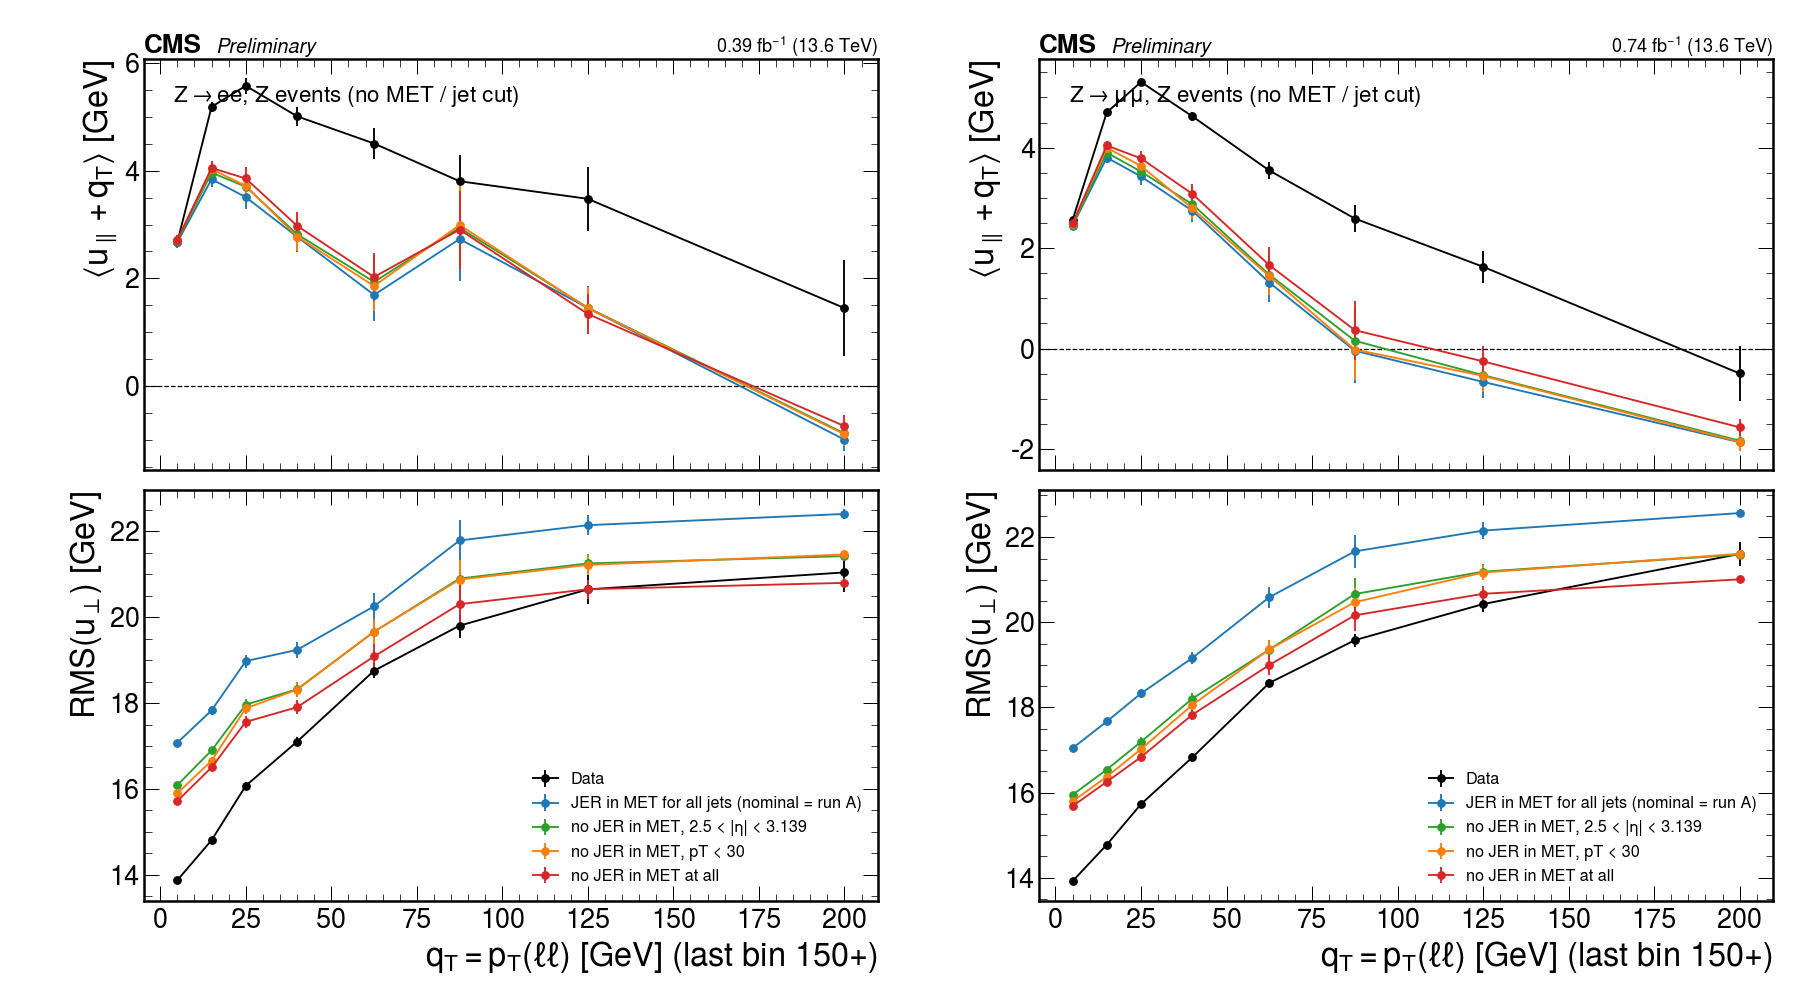
\includegraphics[width=\linewidth]{recoil_Z.png}
\caption{Recoil vs $q_\mathrm{T}$ at the Z stage (no MET or jet cut). Top: response $\langle u_\parallel+q_\mathrm{T}\rangle$.
Bottom: resolution RMS($u_\perp$). Black data, coloured MC versions. Left \Zee, right \Zmm.}
\label{fig:recoilZ}
\end{figure}

\begin{figure}[H]
\centering
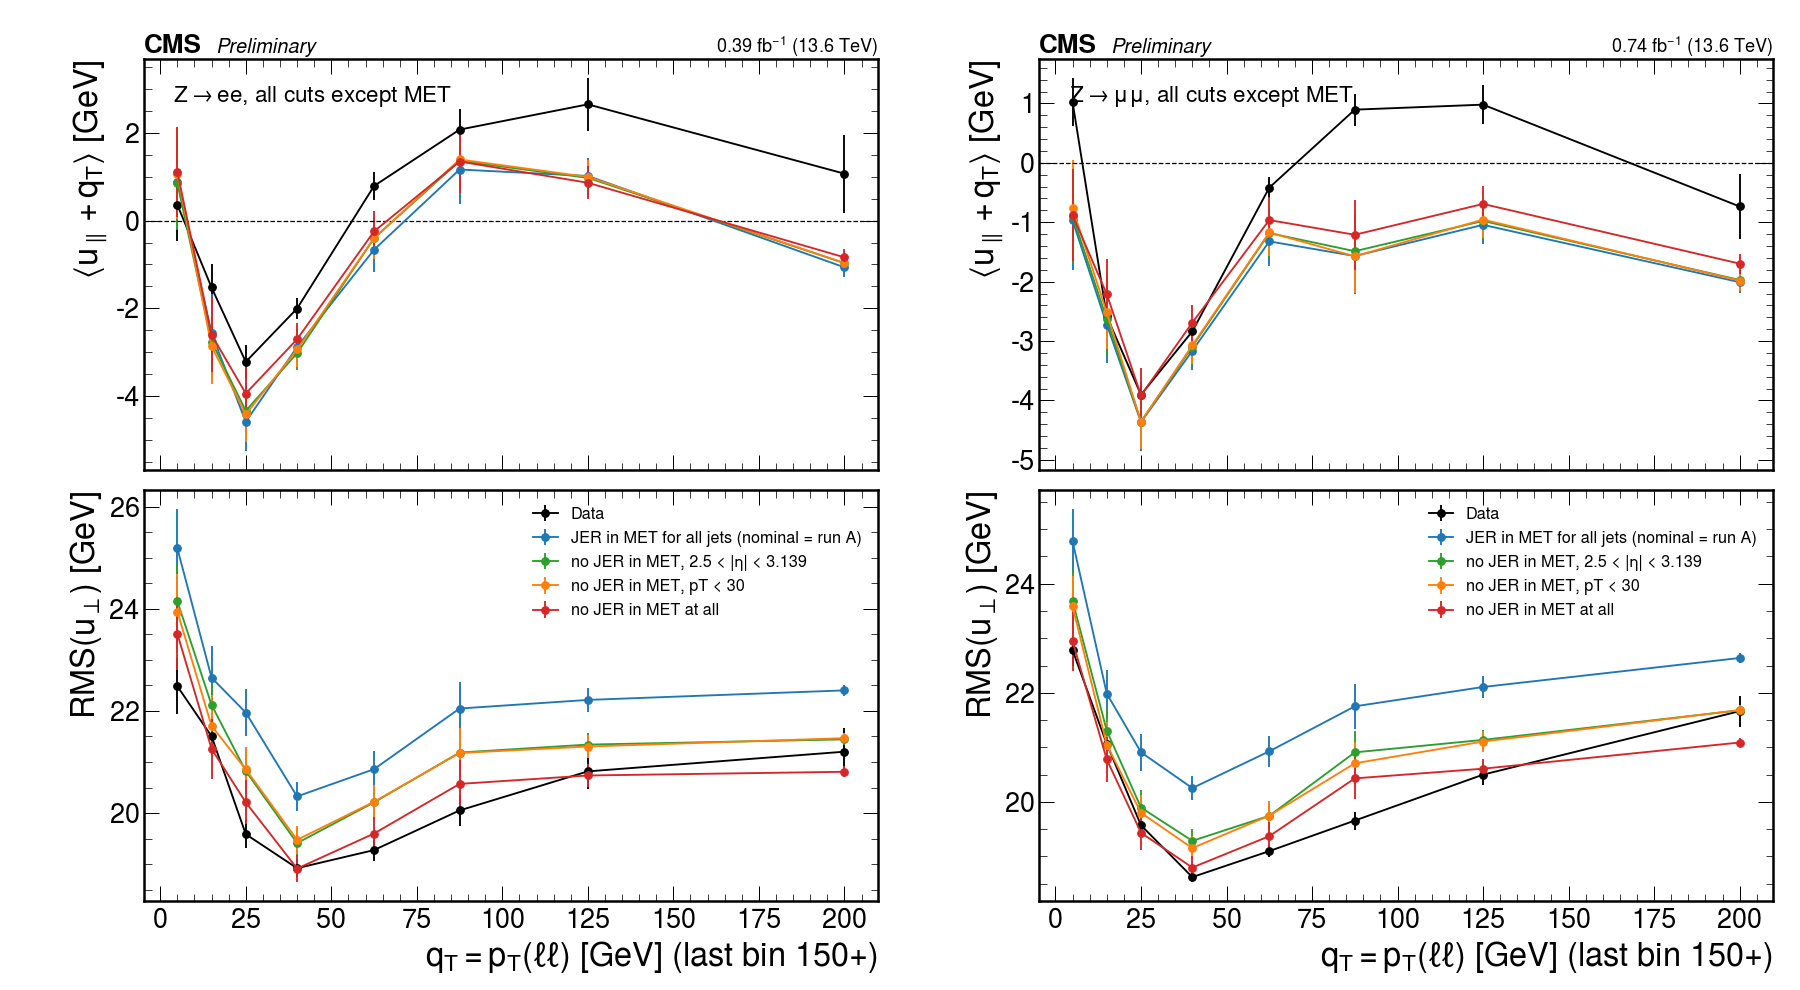
\includegraphics[width=\linewidth]{recoil_Zjet.png}
\caption{As Figure~\ref{fig:recoilZ}, with all cuts except MET (Z + jet).}
\label{fig:recoilZjet}
\end{figure}

\subsection{Numbers}
RMS($u_\perp$) in GeV, columns data / nominal MC / no JER 2.5--3.139 / no JER in MET:
\begin{center}
\small
\begin{tabular}{l l cccc}
\toprule
selection & $q_\mathrm{T}$ [GeV] & data & nominal & no JER 2.5--3.139 & no JER in MET \\
\midrule
Z stage, \Zee & 0--10 & 13.9 & 17.1 & 16.1 & 15.7 \\
 & 30--50 & 17.1 & 19.2 & 18.3 & 17.9 \\
 & 100--150 & 20.6 & 22.1 & 21.3 & 20.7 \\
Z stage, \Zmm & 0--10 & 13.9 & 17.0 & 16.0 & 15.7 \\
 & 30--50 & 16.8 & 19.2 & 18.2 & 17.8 \\
 & 100--150 & 20.4 & 22.2 & 21.2 & 20.7 \\
Z + jet, \Zee & 0--10 & 22.5 & 25.2 & 24.2 & 23.5 \\
 & 30--50 & 18.9 & 20.3 & 19.4 & 18.9 \\
 & 75--100 & 20.1 & 22.1 & 21.2 & 20.6 \\
Z + jet, \Zmm & 0--10 & 22.8 & 24.8 & 23.7 & 22.9 \\
 & 30--50 & 18.6 & 20.3 & 19.3 & 18.8 \\
 & 75--100 & 19.7 & 21.8 & 20.9 & 20.4 \\
\bottomrule
\end{tabular}
\end{center}

\open{The JER explains part of the wider MC recoil, but not all of it}{
\begin{itemize}[leftmargin=12pt]
\item Resolution at the Z stage, low $q_\mathrm{T}$: data 13.9 GeV, nominal MC 17.0--17.1, no JER in the MET 15.7. The JER accounts
for about 1.3 of the 3.1 GeV difference; about 1.8 GeV remain without any JER. Above $q_\mathrm{T}$ = 100 GeV the MC without JER matches data.
\item With a jet required, MC is 1.1--2.7 GeV wider than data with the JER and 0--1 GeV wider without it.
\item Response: at the Z stage, $\langle u_\parallel+q_\mathrm{T}\rangle$ is 1--2.5 GeV higher in data than in every MC version for
$q_\mathrm{T}$ of 10--150 GeV (data recoil measured smaller than MC). The JER versions change it by less than 0.4 GeV. With a jet,
MC follows the shape vs $q_\mathrm{T}$, but above 50 GeV data is 1--2.5 GeV higher in every version.
\item So: there is a second, JER-independent difference in the MC MET at low $q_\mathrm{T}$ (pile-up / unclustered energy, or the
2022 v12 DY MET issue mentioned in the JME talk). It is not studied here.
\end{itemize}}

%======================================================================
\section{Doubts and answers}
\label{sec:doubts}
%======================================================================

This section collects every question that came up or is likely to come up, each answered on its own.

\subsection*{D1. Is the JER smearing already in the NanoAOD, so we apply it twice?}
No. The NanoAOD \texttt{Jet\_pt} is raw \pt{} $\times$ JEC to within 0.3--0.9\%, the MC jet width equals the unsmeared MC resolution,
and the NanoAOD PuppiMET agrees with our JEC-only type-1 MET (Section~\ref{sec:q1}). Our code starts from the raw jet \pt{} and from
RawPuppiMET, so a smeared NanoAOD value could not enter even in principle.

\subsection*{D2. Data/MC looks fine with the JER off. Why not just keep it off?}
Because the JME recipe requires the smearing in MC, for the jets and for the MET (Section~\ref{sec:q2}). With the JER off, the MC jets
are too narrow compared to data; this shows up in our own Z--jet \pt{} balance, which gets worse without JER ($\chi^2$/ndf 40 $\to$ 58
in \Zee, 110 $\to$ 144 in \Zmm). The MET looks better with the JER off because the smearing in the MET is too large for one specific
class of jets (soft forward jets), not because smearing is wrong in general.

\subsection*{D3. Does our type-1 MET follow the JME recipe?}
Yes, step by step (table in Section~\ref{sec:q2}). Two small differences exist (the gen-matching criterion, the \pt{} at which the JEC
is evaluated); both were tested and change the MET by less than 1\%.

\subsection*{D4. Is the stored NanoAOD PuppiMET a better choice than our recomputed one?}
The stored PuppiMET has no JER and uses the production JEC. Compared with our JEC-only MET it gives a 6--10\% larger MET 50--100 fraction,
not smaller. Using it would mean using a MET without JER, i.e.\ the same as switching the JER off in the MET.

\subsection*{D5. Which jets cause the excess?}
About half comes from jets with 2.65 $<$ \aeta{} $<$ 2.853 (JER SF 1.60), mostly with \pt{} $<$ 30 GeV. The rest is spread over all
other jets; no other single class does it (Section~\ref{sec:p1}).

\subsection*{D6. Why do those jets matter so much?}
Their SF is 1.60--1.64 and their MC resolution at 15 GeV is 60--75\%, so the random smearing has a width of about 75\% of the jet \pt.
Every such jet in the MET sum gives the MET an independent random kick (Section~\ref{sec:sf}).

\subsection*{D7. Is it only pile-up jets without a generator jet?}
No. Gen-matched and unmatched jets contribute equally ($R$ = 1.12 and 1.11--1.13). Run C (only gen-matched jets smeared in the MET)
recovered about half of the deficit (0.84), consistent with this.

\subsection*{D8. Is it the CorrT1METJet collection?}
Partly. Smearing only the CorrT1METJet jets gives $R$ = 1.12; removing their smearing moves data/MC at MET 50--100 from 0.70 to only 0.77 / 0.75.

\subsection*{D9. Is it the jets we select for the analysis?}
No. Smearing only jets of the selected type (\pt{} $>$ 30 GeV, \aeta{} $<$ 2.5) gives $R$ = 1.08. In Phase 2 the selected jets are smeared in
every version, and the deficit still closes when the MET smearing of other jets is removed.

\subsection*{D10. Can the SF uncertainty cover the effect?}
No. At $-1\sigma$ the SFs are still 1.45 (2.65--2.853) and 1.36 (2.853--2.964), giving a random smearing of 63--69\% at 15 GeV instead
of 75\%. The relative uncertainty is 9.6\% (not $\pm$0.10 absolute, as said earlier). A full run with the JER-down variation was not made.

\subsection*{D11. Does the MET XY correction play a role?}
No. It shifts the MET by about 1 GeV and makes the MET $\phi$ flatter; it is applied identically to every version and was already
shown (16 November) to have no effect on the MET $>$ 50 region.

\subsection*{D12. Why were the data not rerun?}
Data have no JER, so the data MET is the same in every version. Using the data histograms of run A is exact, not an approximation.

\subsection*{D13. Why does data/MC below 50 GeV get worse when the MET gets better?}
Because the MC yield is fixed: the smearing only moves MC events across the cut. Less smearing keeps more MC events below 50 GeV, so
data/MC there drops by 1.5--2.7\%. With no JER in the MET, data/MC is flat at 0.94--0.95: the shape is right, and an overall 5\%
normalisation remains (not studied here).

\subsection*{D14. Does any of this matter for the Z+b / Z+c ratio?}
A little. The MC b/c-tag yield ratio moves by $<$1\% at Loose, up to 2.7\% at Medium and up to about 3\% at Tight
(Section~\ref{sec:bc}). This is about the size of the current data statistical error on the ratio. The data/MC in all tag regions
shifts together with the inclusive selection, so the effect is mostly common to b and c.

\subsection*{D15. Are the Phase 1 numbers reliable, given the simplified selection?}
Yes for this purpose: they predicted 0.83 / 0.86 for the 2.5--3.139 version, and the full run measured 0.82 / 0.84. Phase 1 reproduced
the full-run effect of JER on/off (factor 1.37--1.39 vs 1.38).

\subsection*{D16. Is the agreement in the full run exact by construction or a real check?}
Version ``all'' was checked against the framework MET in every event (0 of 2.8 million events differ by more than 0.01 GeV) and against
run A's histograms (identical). So the versions differ from the nominal only by the intended change.

\subsection*{D17. Is everything fixed if we remove the forward smearing from the MET?}
No. About half of the MET 50--100 deficit remains (0.82--0.84), the MC recoil remains wider than data at low $q_\mathrm{T}$ even with no
JER at all, and the recoil response differs by 1--2.5 GeV independently of the JER (Section~\ref{sec:recoil}).

\subsection*{D18. Could the 2022 NanoAODv12 DY sample itself be part of the problem?}
Possibly. The JME talk of 2 February reports that 2022 v12 DY samples have a problematic MET resolution, which NanoAODv15 does not show.
This could be part of the JER-independent recoil difference. Not tested: it needs another DY sample or a v15 comparison.

\subsection*{D19. How significant are the results with 20 files per sample?}
The MET 50--100 data/MC changes (0.70 $\to$ 0.82--0.95) are 3.5--8.5 standard deviations of the data/MC error, and the errors of different
versions are strongly correlated (same data, mostly the same MC events), so the differences between versions are more precise than
the quoted errors. The 100--200 GeV bin (errors 7--17\%) is not conclusive.

\subsection*{D20. Is this specific to Summer22?}
Only Summer22 was studied. The JER SFs of other campaigns have their own \aeta{} structure; the same run can be repeated for
Summer22EE, Summer23 and Summer23BPix.

%======================================================================
\section{Conclusions, what is not fixed, and next steps}
\label{sec:concl}
%======================================================================

\subsection{Conclusions}
\begin{enumerate}
\item No double counting: the NanoAOD has no JER, and we apply it once, in MC, to the jets and to the type-1 MET, as JME recommends.
\item The MET 50--100 GeV deficit is caused by the JER smearing of the MC MET. About half comes from soft jets at 2.5 $<$ \aeta{} $<$ 3.139,
where the JER SFs are 1.2--1.64 and the MC resolution at 15 GeV is 50--75\%. The rest is spread over the other jets.
\item The MC-only study and the full run agree (0.83 / 0.86 predicted, 0.82 / 0.84 measured).
\item With no JER in the MET, the MC describes the MET shape (data/MC flat at 0.94--0.95).
\item For the Z+b / Z+c ratio the MET choice matters at the 1--3\% level: below 1\% at Loose and up to about 3\% at Tight.
\end{enumerate}

\subsection{What is not fixed}
\begin{itemize}
\item The MC recoil is about 2 GeV wider than data at low $p_\mathrm{T}(\ell\ell)$ even with no JER at all.
\item The recoil response differs by 1--2.5 GeV between data and MC, independently of the JER.
\item The overall data/MC normalisation of about 0.95 (with no JER in the MET) is not understood yet.
\item The MET 100--200 GeV bin has too few events to conclude.
\item Only Summer22, only 20 files per sample, statistical errors only.
\end{itemize}

\subsection{Proposal and next steps}
\begin{enumerate}
\item \textbf{Keep the JME recipe as nominal} (run A: JER on for the jets and the MET).
\item \textbf{Use the MET versions as a systematic uncertainty} on the b/c ratio from the MET cut: the change when the JER is removed
from the MET for 2.5 $<$ \aeta{} $<$ 3.139, or from the MET entirely, whichever is larger. This keeps the recipe and covers the region
where it does not describe the data.
\item \textbf{Ask JME} whether the SF of 1.60--1.64 for 2.65 $<$ \aeta{} $<$ 2.964 is meant to be used for jets below 30 GeV and for
the low-\pt{} jets that enter the MET. Show them Figure~\ref{fig:p1} and the MET 50--100 numbers.
\item \textbf{Understand the remaining recoil difference}: pile-up in the Z events (number of vertices, $\rho$), the unclustered PUPPI part
of the MET, and a comparison with another DY sample (JME remark on 2022 v12 DY).
\item \textbf{More statistics and other eras}, if wanted: the same run for Summer22EE, Summer23 and Summer23BPix.
\end{enumerate}

\appendix
\sloppy
%======================================================================
\section{Analysis setup}
\label{app:setup}
%======================================================================
All corrections are from the CMS jsonPOG files (\texttt{/cvmfs/cms-griddata.cern.ch/cat/metadata}), Summer22 versions.

\textbf{Data.} 2022 runs C--D, EGamma and Muon datasets, 22Sep2023 reprocessing, NanoAODv12. Certified lumisections only (golden JSON
Cert\_Collisions2022\_355100\_362760). Test sample: 20 files per channel = 389 pb$^{-1}$ (ee) and 742 pb$^{-1}$ ($\mu\mu$), measured with
brilcalc (normtag\_PHYSICS) on the lumisections actually read.

\textbf{Simulation (Run3Summer22, NanoAODv12).} Drell--Yan: DYto2L-2Jets, MadGraph5\_aMC@NLO with FxFx merging (0, 1, 2 partons at NLO),
m($\ell\ell$) $>$ 50 GeV; inclusive sample used for generator $p_\mathrm{T}(\ell\ell)$ $<$ 100 GeV, $p_\mathrm{T}(\ell\ell)$-binned samples
above (100--200, 200--400, 400--600, $>$600). Backgrounds: $t\bar t\to 2\ell2\nu$ (POWHEG), WW, WZ, ZZ (Pythia8). Each sample scaled to
cross section $\times$ luminosity / sum of generator weights; 20 files per sample.

\textbf{Triggers.} \Zee: HLT\_Ele30\_WPTight\_Gsf. \Zmm: HLT\_IsoMu24.

\textbf{Leptons.} Electrons: \pt{} $>$ 25 GeV, \aeta{} $<$ 2.4, cut-based Tight ID, barrel--endcap gap 1.442 $<|\eta_\mathrm{SC}|<$ 1.566
removed, $|d_{xy}|<$ 0.05 (0.1) cm and $|d_z|<$ 0.1 (0.2) cm in the barrel (endcap). Muons: \pt{} $>$ 26 GeV, \aeta{} $<$ 2.4, Tight ID,
PF isolation ($\Delta R$ = 0.4) $<$ 0.15.

\textbf{Z + jet selection (in this order).} Trigger; two leptons of the channel, leading lepton \pt{} $>$ 35 GeV; opposite charge;
71 $<$ m($\ell\ell$) $<$ 111 GeV; type-1 PUPPI MET $<$ 50 GeV; at least one AK4 PUPPI jet with \pt{} $>$ 30 GeV, \aeta{} $<$ 2.5,
Tight-lepton-veto ID (with the NanoAODv12 fix), $\Delta R>$ 0.4 from the leptons. The leading jet is studied and tagged.

\textbf{Jets and MET.} JEC Summer22\_22Sep2023\_V4 (data per era and MC); JER Summer22\_22Sep2023\_JRV2 (MC). Type-1 PUPPI MET recomputed
with the corrected jets. PUPPI MET XY correction (JME met\_xyCorrections\_2022, epoch 2022). Jet veto map Summer22\_23Sep2023\_RunCD\_V1:
event dropped if a jet (\pt{} $>$ 15 GeV, tight ID, EM fraction $<$ 0.9, no muon nearby) is in a vetoed region.

\textbf{Lepton corrections.} Electron energy scale (data) and smearing (MC), EGM. Muon momentum scale (data) and smearing (MC), MUO.

\textbf{Event cleaning.} MET filters in data and MC: goodVertices, globalSuperTightHalo2016, EcalDeadCellTriggerPrimitive, BadPFMuon,
BadPFMuonDz, hfNoisyHits, eeBadSc.

\textbf{Event weights in MC.} Pile-up (LUM puWeights, 2022 C--D golden profile, 69.2 mb). Electron reconstruction and Tight ID SFs
(EGM 2022 Re-reco BCD). Muon Tight ID SF (NUM\_TightID\_DEN\_TrackerMuons) and Tight isolation SF (NUM\_TightPFIso\_DEN\_TightID).
Trigger SF for either lepton firing: $[1-(1-\epsilon^1_\mathrm{data})(1-\epsilon^2_\mathrm{data})]/[1-(1-\epsilon^1_\mathrm{MC})(1-\epsilon^2_\mathrm{MC})]$
with the POG efficiencies. DY Z \pt{} weights (not a POG correction): DY MC reweighted in bins of reconstructed $p_\mathrm{T}(\ell\ell)$,
weights from \Zmm{} data/MC before the MET and jet cuts, total DY yield unchanged, applied in both channels. No L1 prefiring weight (not needed in Run 3).

\textbf{b and c tagging (leading jet).} ParticleNet, DeepJet, RobustParT; official BTV Summer22 Loose/Medium/Tight working points.
b-tag: B score $>$ cut; c-tag: CvL $>$ cut and CvB $>$ cut (separate selections). MC tagged jets weighted by the BTV SF for their true
flavour (hadronFlavour). This report uses ParticleNet.

\textbf{Uncertainties.} Statistical only (data and MC). SFs at their central values; systematic uncertainties not included yet.
Software: coffea 0.7, BTVNanoCommissioning (Zb\_Zc\_ratio workflow), correctionlib.

%======================================================================
\section{Files, code and how to reproduce}
%======================================================================
Repository: \texttt{Pranjal-Srivastava-2023/BTVNanoCommissioning}, branch \texttt{coffea\_machine}.
\begin{center}
\small
\begin{tabular}{>{\raggedright}p{4.0cm} >{\raggedright\arraybackslash}p{11.6cm}}
\toprule
what & where \\
\midrule
JME documentation and talks & \path{src/BTVNanoCommissioning/*.pdf} \\
type-1 MET and JER code & \path{src/BTVNanoCommissioning/utils/correction.py} (\path{JME_shifts}, \path{calc_T1_MET}, \path{get_JER}) \\
MET versions in the workflow & \path{workflows/Zb_Zc_ratio.py} (\path{MET_VARIANTS}, \path{common_shifts_metvar}, \path{fill_metvar}); \path{workflows/__init__.py}: \path{Zb_Zc_ratio_metvar} \\
Phase 1 (MC only) & \path{study_zbzc_met_jer_split.py}, \path{plot_zbzc_met_jer_split.py} $\to$ \path{hists_zbzc_run3_metsplit/Summer22/} \\
Phase 2 run & \path{hists_zbzc_run3_metvar/Summer22/zbzc_run3/} (coffea, not in git), logs \path{logs_zbzc_run3_metvar/} \\
Phase 2 tables and plots & \path{plot_zbzc_metvar.py} $\to$ \path{hists_zbzc_run3_metvar/Summer22/metvar/metvar.{txt,json\}} + png \\
Slides & \path{hists_zbzc_run3_metvar/Summer22/slides_zbzc_metvar_Summer22.{pdf,pptx\}} \\
This report & \path{hists_zbzc_run3_metvar/Summer22/report/report_MET50_JER_Summer22.{tex,pdf\}} \\
Earlier runs A, B, C & \path{hists_zbzc_run3_metxy}, \path{_metxy_nojer}, \path{_metxy_jermatched} (Summer22) \\
Running notes & \path{NOTES_Zb_Zc_ratio_run3.md} \\
\bottomrule
\end{tabular}
\end{center}

\textbf{Reproduce.}
{\footnotesize
\begin{verbatim}
# Phase 1 (MC only, ~15 min, local)
python study_zbzc_met_jer_split.py hists_zbzc_run3_metsplit/Summer22 30,15,10,6,4
python plot_zbzc_met_jer_split.py hists_zbzc_run3_metsplit/Summer22
# Phase 2: run workflow Zb_Zc_ratio_metvar on the MC samples (20 files each),
# then link run A data and make the tables, plots and slides
bash postprocess_zbzc_metvar.sh
python plot_zbzc_metvar.py
PYTHONPATH=$PWD python make_zbzc_metvar_slides_pdf.py
# this report
cd hists_zbzc_run3_metvar/Summer22/report
pdflatex report_MET50_JER_Summer22.tex   # run twice
\end{verbatim}
}

\begin{figure}[H]
\centering
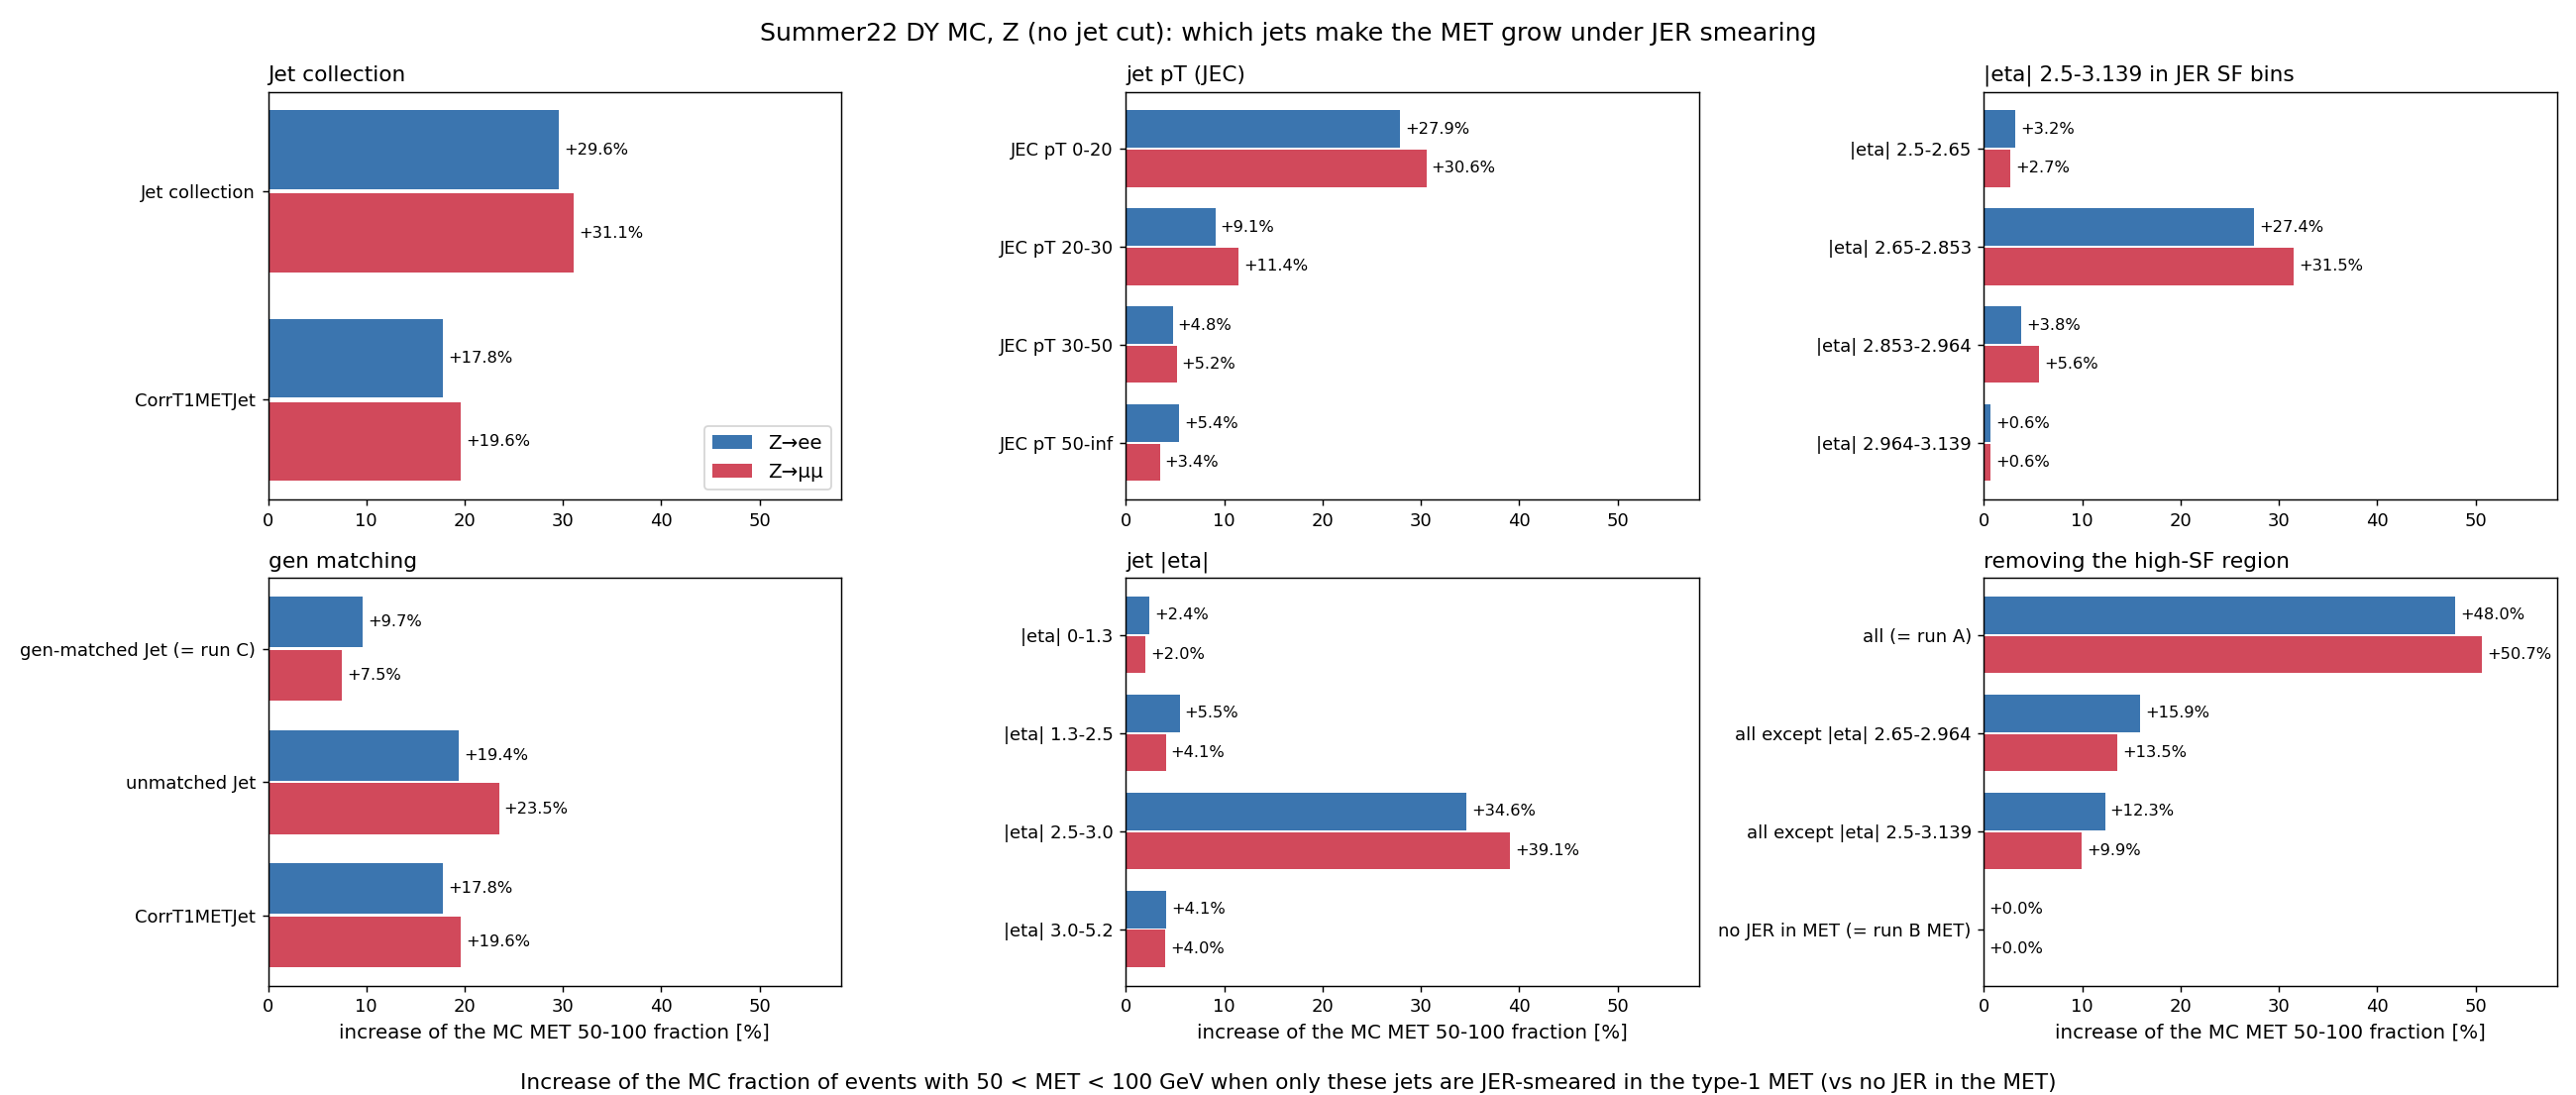
\includegraphics[width=\linewidth]{met_jer_split_z.png}
\caption{Phase 1 at the Z stage (no jet or MET cut), for comparison with Figure~\ref{fig:p1}.}
\end{figure}

\end{document}
